\documentclass[letterpaper]{article}

\usepackage{natbib,alifexi}
\usepackage{amsmath}
\usepackage[french]{babel}
\usepackage[utf8]{inputenc}
\usepackage{hyperref}
\usepackage{amsfonts}
\usepackage{graphicx}
\usepackage{blkarray}
\usepackage{tikz}
\usetikzlibrary{automata, positioning}

\newcommand{\colornode}[1][]{\node[state,
	    align=center,
	    text=gray!40!black,
	    draw=gray,
	    fill=gray!20!white,{#1}]}
\newcommand{\bigcolornode}[1][]{\node[state,
	    align=center,
	    text=gray!40!black,
	    draw=gray,
	    fill=gray!20!white,
	    text width=1.7cm,{#1}]}

\newcommand{\drawedge}{\draw[every loop, line width=0.4mm, fill=gray, draw=gray]}

\newcommand*{\fullref}[1]{\hyperref[{#1}]{\autoref*{#1} \nameref*{#1}}}


\title{Etude du Monopoly via les chaînes de Markov}
\author{Rémy Detobel\\
Mickael Randour\\
\mbox{}\\
Université Libre de Bruxelles, Bruxelles, Belgique \\
rdetobel@ulb.ac.be}


% =-=-=-=-=-=-=-=-= TODO GENERAL =-=-=-=-=-=-=-=-=
% - Bibliographie (revoir l'affichage, la mise en page)
% - Résultats
% - Conclusion

% TODO question: lorsque l'on a fait 2 doubles et qu'on a une carte chance qui nous déplace... On a
% toujours 2 doubles à notre actif ou pas ? (de préférence oui, on perd)


\begin{document}
\maketitle

\begin{abstract}
  Modélisation et étude du Monopoly à travers les chaînes de Markov.
  Les concepts principaux de ce modèle qu'est une chaîne de Markov,
  seront présentés et expliqués.  Les différents choix permettant 
  d'adapter le Monopoly afin qu'il puisse être modélisé comme une chaîne 
  de Markov seront également expliqués.  Enfin, une description de 
  l'application et des résultats récupérés par l'implémentation de cette 
  modélisation sera également faite et permettra de déterminer les cases 
  les plus fréquentées ainsi que les cases les plus rentables.
  % beaucoup de répétition de ``présenter'' et ``expliqué''
\end{abstract}

%%%%%%%%%%%%%% SECTION %%%%%%%%%%%%%%
\section{Introduction}
  Contrairement aux idées reçues, chaque case du Monopoly n'a pas la même
  probabilité d'être visitée.  Il est donc intéressant d'étudier quelles sont
  les cases les plus fréquentées mais également quelles seraient les cases
  les plus rentables.  Dans cette idée, il est possible de modéliser
  le Monopoly à travers les chaînes de Markov.  Mais avant cela, il est 
  important de bien définir les chaînes de Markov ainsi que leurs propriétés.
  Les explications concernant ce modèle sont en grande partie basées 
  sur le cours de \citet{COURS}.
  Pour pouvoir modéliser le Monopoly comme étant une chaîne de Markov, 
  les règles du jeu doivent être clairement définies et des choix doivent
  être faits.  Ceux-ci seront donc expliqués et justifiés dans cet article.
  Les résultats trouvés suite à cette modélisation seront présentés afin
  de trouver, au final, les cases les plus visitées mais également les cases
  les plus rentables.
  % TODO ajouter des informations à l'intro (peut être plus conséquent)
  
  
%%%%%%%%%%%%%% SECTION %%%%%%%%%%%%%%
\section{Approche théorique}
  
  \subsection{Les chaînes de Markov}
    \label{def_chaine_markov}
    Une chaîne de Markov est une structure de données qui permet de modéliser l'évolution
    de l'état d'un système aléatoire.  Les chaînes de Markov sont basées sur le 
    fait que l'état actuel du système dépend uniquement de l'état précédent.
    Cette propriété peut être appelée ``propriété de Markov''.  Une chaîne de
    Markov est donc composée d'états et de liens entre ces différents états caractérisés
    par une certaine probabilité de passer d'un état A à un état B.
    Cette probabilité sera décrite plus en détail dans le point \ref{probabilite}.
    Il est possible de représenter une chaîne de Markov de plusieurs manières différentes.
    Dans la littérature (comme par exemple dans le cours \citet{COURS}), on utilisera 
    plus souvent la notation matricielle, qui définit la chaîne de Markov $\mathcal{M}$ 
    telle que:
    $$\mathcal{M} = (S, \mathbf{P}, \iota_{init})$$
    Où $S$ représente l'ensemble de tous les états possibles, $\mathbf{P}$ une matrice $S \times S$
    où chaque élément est compris entre 0 et 1 et où cette valeur représente la probabilité 
    de passer d'un état à un autre (respectivement, l'état correspondant à la ligne et à la colonne).
    On appellera cette matrice $\mathbf{P}$ la \textit{matrice de transition}.
    $\iota_{init}$ est une matrice colonne où chaque ligne représente un état et la valeur
    associée représente la probabilité de commencer par cet état.  On peut retrouver d'autres
    variables dans la littérature (comme $AP$ et $L$ par exemple pour associer des propositions 
    atomiques aux états) mais celles-ci ne seront pas utiles dans cet article.
    Il est également possible de représenter une chaîne de Markov sous forme
    d'un graphe dirigé où chaque nœud représente un état et chaque arête est pondérée
    en fonction de la probabilité de passer d'un état à un autre.
    Notons également que les chaînes de Markov peuvent être utilisées
    dans un temps discret ou dans un temps continu.  Cependant, la modélisation
    du Monopoly n’inclura pas de temps continu et cet article traitera donc uniquement
    du temps discret.
    % TODO voir pour définir AP et L en 2 phrases
    
  \subsection{Exemple de chaîne de Markov}
    \label{exemple}
    Afin d'illustrer les notions liées aux chaînes de Markov, cet article se 
    basera sur un exemple représentant les différents états que peut avoir 
    un avion.  On va donc ici considérer qu'un avion pourra avoir 6 états 
    différents: \textit{en vol} (noté \textit{vol}), \textit{atterrissage} 
    (noté \textit{att.}), \textit{décollage} (noté \textit{dec.}), 
    \textit{au sol}, \textit{contrôle} (noté \textit{ctr.})
    et \textit{hors service} (noté \textit{h.s.}).
    On va considérer que lors de l'\textit{atterrissage}, il y a une chance sur 
    3 pour qu'un voyant indique au pilote qu'un \textit{contrôle} est 
    nécessaire. On remarque également qu'il y a une chance sur 10 que 
    l'avion ne passe pas le \textit{contrôle} et soit considéré comme 
    \textit{hors service}.  On considérera également que tous les avions commencent
    avec l'état \textit{au sol}.
    
    \subsubsection{Représentation matriciel}
      Comme vu au point \ref{def_chaine_markov}, il est possible de représenter une
      chaîne de Markov comme étant:
      $$\mathcal{M} = (S, \mathbf{P}, \iota_{init})$$
      Pour notre exemple on aura donc:
      $$S = \{vol, dec., att., sol, ctr., h.s.\} $$
      $$ \mathbf{P} = 
	\begin{blockarray}{ccccccc}
	& vol & dec. & att. & sol & ctr. & h.s. \\
	  \begin{block}{c(cccccc)}
	    vol  & 0 & 0 & 1 & 0    & 0   & 0    \\
	    dec. & 1 & 0 & 0 & 0    & 0   & 0    \\
	    att. & 0 & 0 & 0 & 2/3  & 1/3 & 0    \\
	    sol  & 0 & 1 & 0 & 0    & 0   & 0    \\
	    ctr. & 0 & 0 & 0 & 9/10 & 0   & 1/10 \\
	    h.s. & 0 & 0 & 0 & 0    & 0   & 1    \\
	  \end{block}
	\end{blockarray}
      $$
      $$\iota_{init} = 
	\begin{blockarray}{cc}
	  \begin{block}{( c ) c}
	    0 & vol \\
	    0 & dec.\\
	    0 & att.\\
	    1 & sol\\
	    0 & ctr.\\
	    0 & h.s.\\
	  \end{block}
	\end{blockarray}
      $$
      
    \subsubsection{Représentation graphique}
      Il est également possible de représenter cette chaîne de Markov comme
      étant un graphe dirigé (cfr point \ref{def_chaine_markov}):
      \begin{center}
	\begin{tikzpicture}
	  % Draw the states
	  \colornode[text width=1.7cm] (vol) {En vol};
	  
	  \colornode[below left=of vol] (att) {Atterrissage};
	  \bigcolornode[below right=of vol] (dec) {Décollage};
	  
	  \bigcolornode[below right=of att] (sol) {Au sol};

	  \bigcolornode[below left=of sol] (ctr) {Contrôle};
	  \colornode[right=of ctr] (hs) {Hors service};

	  % Connect the states with arrows
	  \drawedge
	    (vol) edge[bend right, auto=right] node {1} (att)
	    (dec) edge[bend right, auto=right] node {1} (vol)
	    (sol) edge[bend right, auto=right] node {1} (dec)
	    (att) edge[bend right, auto=right] node {2/3} (sol)
	    (att) edge[bend right, auto=right] node {1/3} (ctr)
	    (ctr) edge[bend right, auto=left] node {9/10} (sol)
	    (ctr) edge[bend right, auto=right] node {1/10} (hs)
	    (hs) edge[loop right] node {1} (hs);
	  \draw [->, line width=0.4mm, fill=gray, draw=gray] (1.6,-5.4) -- (sol);
	\end{tikzpicture}
      \end{center}
    
  \subsection{Probabilité}
    \label{probabilite}
    La notion de probabilité peut se définir de plusieurs manières différentes 
    et de nombreux ouvrages (comme par exemple celui de \citet{IP}) décrivent 
    de manière très détaillée la notion de probabilité.  Dans ces ouvrages, on
    traite souvent des espaces de probabilité, qui demandent une approche très 
    abstraite et rigoureuse.  Cependant dans cet article, l'approche
    fréquentielle inspirée des statistiques est suffisante.
    On définit donc la probabilité d'un événement aléatoire par la limite
    de la fréquence d’occurrence d'un événement pour un nombre d'expériences
    tendant vers l'infini.  De manière plus formelle, on peut décrire ce
    comportement comme $X$ étant une expérience aléatoire ayant
    $$X_i \mid i \in I $$
    pour résultats possibles, avec $I$ un ensemble d'indices (qui peuvent 
    être fini, infini dénombrable ou infini non-dénombrable).  On définit
    la probabilité du résultat $X_i$ pour $i \in I$ par:
    $$\lim_{n \to \infty}\frac {X_i(n)}n,$$
    avec $X_i(n)$, le nombre d'occurrence du résultat $X_i$ lors de
    $n$ itérations de l'expérience $X$.  On note cette valeur
    $\mathbb P[X = X_i]$, si cette limite existe.
    % TODO lier ceci avec le reste du rapport
    % QUESTION Randour: ajouter ceci ?
    % Remarque : il est important de demander que la limite existe, par exemple 
    % si le nombre d'occurrences est sous la forme $X(n) = n\cos(n)$, on remarque 
    % qu'il est impossible de définir une probabilité, alors qu'une fréquence a un sens.
    
  \subsection{Simuler les changements d'état}
    Une chaîne de Markov permet donc d'estimer la probabilité de l'état
    futur d'un système uniquement en se basant sur l'état actuel du système.
    Dans cette idée, la matrice de transition $\mathbf{P}$ représente tous les
    déplacements d'une unité possible.  Si maintenant on veut connaître
    les états accessibles depuis notre état actuel après deux unités de temps,
    il suffit d'élever la matrice de transition au carré.  Si l'on reprend
    notre exemple, on aura donc:
    \begin{align*}
    \mathbf{P}^2 &= 
      \begin{pmatrix}
	0 & 0 & 1 & 0    & 0   & 0    \\
	1 & 0 & 0 & 0    & 0   & 0    \\
	0 & 0 & 0 & 2/3  & 1/3 & 0    \\
	0 & 1 & 0 & 0    & 0   & 0    \\
	0 & 0 & 0 & 9/10 & 0   & 1/10 \\
	0 & 0 & 0 & 0    & 0   & 1    \\
      \end{pmatrix}^2\\
      &= 
      \begin{pmatrix}
        0 & 0    & 0 & 2/3  & 1/3 & 0    \\
	0 & 0    & 1 & 0    & 0   & 0    \\
	0 & 2/3  & 0 & 3/10 & 0   & 1/30 \\
	1 & 0    & 0 & 0    & 0   & 0    \\
	0 & 9/10 & 0 & 0    & 0   & 1/10 \\
	0 & 0    & 0 & 0    & 0   & 1    \\
      \end{pmatrix}
    \end{align*}
    % TODO A voir si c'est clair
    On remarque donc qu'après 2 déplacements depuis le premier état (première
    ligne), il sera possible d'atteindre le 4 et 5\up{ème} état (avec 
    respectivement une probabilité de $2/3$ et $1/3$).  Ce comportement est
    très simple à voir dans cet exemple, car l'état succédant l'état 1 est
    obligatoirement le 3\up{ème} état.  Il est donc normal qu'après 2 tours,
    on retrouve les probabilités de déplacement du troisième état.
    
  \subsection{Propriété d'une chaîne de Markov}
    On peut remarquer que la somme de tous les éléments de chaque ligne de la
    matrice de transition fait $1$.  Ce phénomène peut également être vu
    sur la représentation graphique de la chaîne de Markov où la somme de chaque
    arête quittant un nœud (un état donc) vaut $1$.  Par exemple, si l'on se
    concentre sur l'état \textit{att.} (sur la représentation matricielle il s'agit donc 
    de la 3\up{ème} ligne), on a bien: $2/3 + 1/3 + 0$ qui vaut bien $1$.  De manière 
    plus formelle, cette caractéristique peut être notée telle que pour une matrice
    $\mathcal{M}$ (définie au point \ref{def_chaine_markov}) et pour tout état $s \in S$:
    $$\sum\limits_{s' \in S} \mathbf{P}(s, s') = 1$$
    Où $\mathbf{P}(s, s')$ représente la probabilité (présente dans la matrice de
    transition) de passer de l'état $s$ à l'état $s'$.  Cette caractéristique est
    toujours vraie par définition d'une chaîne de Markov mais également par définition
    d'une probabilité.
    En effet, la matrice $\mathbf{P}$ contient toutes les relations possibles entre
    tous les états du système ($S \times S$).  Une ligne représente donc toutes les 
    relations possibles entre un état (définit par la ligne actuelle) et tous les autres
    états du système (les $S$ colonnes).  La probabilité de passer de l'état actuel
    à n'importe quel autre état du système est donc égale à $1$ (par définition d'une probabilité).
    Avec ce même raisonnement, il est logique de se rendre compte que la matrice
    de distribution initiale possède les mêmes caractéristiques:
    $$\sum\limits_{s \in S} \iota_{init}(s) = 1$$
    
  \subsection{Notation des chaînes des Markov}
    Certaines chaînes de Markov ont différentes structures et certains
    sous-ensembles d'états possèdent des caractéristiques particulières.
    Ces ensembles sont donc notés via différentes abréviations.  Ces différentes
    abréviations et concepts sont utilisés dans plusieurs articles scientifiques
    comme par exemple dans le livre de \citet{ModelChecking} ou dans le cours
    \citet{COURS}.  Pour formaliser ces différents concepts, on définit 
    une chaîne de Markov $\mathcal{M}(S, \mathbf{P}, \iota_{init})$ 
    (comme vu au point \ref{def_chaine_markov}) ainsi qu'un sous-ensemble $T$ de $S$.
    
    \subsubsection{Fortement connexe}
      Ce sous-ensemble $T$ sera défini comme \textit{fortement connexe} si
      pour chaque paire d'état $(s, t)$ telle que $s, t \in T$, il existe un
      chemin $s_0, s_1, ..., s_n$ tel que $s_i \in T$ pour $0 \leq i \leq n$, 
      $s_0 = s$ et $s_n = t$.\\
      Dans l'exemple présenté au point \ref{exemple}, une composante fortement
      connexe pourrait être: $\{vol, att., dec., sol\}$.
      
    \subsubsection{Composante fortement connexe}
      Une composante fortement connexe est abrégée \textit{SCC} (``Strongly
      Conntected Component'' en anglais).  Le sous-ensemble $T$ est une 
      composante fortement connexe lorsque celui-ci est fortement connexe et
      que l'ajout d'un élément dans ce sous-ensemble violerait les propriétés
      définies par un ensemble fortement connexe.
      
    \subsubsection{BSCC}
      \label{bscc}
      \textit{BSCC} signifie ``Bottom Strongly Connected Component'' en anglais.
      Une \textit{BSCC} de $\mathcal{M}$ est une composante fortement connexe 
      (SCC) $T$ tel qu'aucun état en dehors de $T$ n'est accessible.  De manière
      plus formelle, cela signifie que $\forall s \in T$:
      $$\sum\limits_{t \in T} \mathbf{P}(s, t) = 1$$
      L'exemple du point \ref{exemple} a pour seul BSCC: $\{h.s.\}$ (qui 
      est donc uniquement composé d'un seul état).
      La propriété précédente nous apprend donc que lorsqu'un avion sera
      considéré comme \textit{hors service}, il n'y a aucun moyen de quitter
      cet état.  En effet, comme définit ci-dessus, tous les changements
      d'états pouvant être fait depuis un état présent dans un BSCC sont dirigés
      vers état étant lui même présent dans ce BSCC.
      
%       De manière intuitive, on pourra donc dire que lorsqu'une chaîne de Markov
%       se retrouve dans un état présent dans un BSCC aura à partir de ce moment
%       là, tous ses états également présent dans ce BSCC.
%       
%       
%       Cette propriété nous indique donc que pour tout état $s$ présent dans
%       ce BSCC, l'évolution de l'état de la chaîne de Markov 
%       
%       Il est important de noter qu'une fois que l'état actuel se retrouve dans une
%       BSCC, il est impossible d'en sortir.  Cela signifie qu'après un nombre fini
%       ou infini dénombrable d'étapes, on sera toujours dans un état présent dans le BSCC
%       pour autant que l'on ait commencé dans ce BSCC.\\
%       L'exemple du point \ref{exemple} a pour seul BSCC: $\{h.s.\}$ (qui 
%       est donc uniquement composé d'un seul état).
  
  \subsection{Distribution stationnaire}
    \label{distribution_stationnaire}
    Comme vu au point \ref{bscc}, la probabilité de se retrouver dans un état
    présent dans un BSCC après un nombre fini ou infini dénombrable d'étape est
    toujours de 1 (pour autant que l'on ait commencé dans un état lui-même présent
    dans ce BSCC).  Remarquons cependant que chaque état présent dans ce BSCC n'a 
    pas la même probabilité d'être visité.  En effet, certains états seront 
    visités plus souvent que d'autres.
    On définit la distribution stationnaire comme étant un vecteur de probabilité
    $\mathbf{v}$ tel que:
    $$\mathbf{v}\mathbf{P} = \mathbf{v}$$
    et où pour chaque élément $\mathbf{v}_i \in \mathbf{v}, \mathbf{v}_i \in [0, 1]$.
    Par définition d'un BSCC, la somme des probabilités de chaque état doit valoir 1
    (car après un nombre fini ou infini dénombrable d'étapes, on sera toujours dans
    état présent dans ce même BSCC), on peut donc écrire:
    $$\sum\limits_{\mathbf{v}_i \in \mathbf{v}} \mathbf{v}_i = 1$$
    
    \subsubsection{Calcul de la distribution stationnaire}
      Nous allons définir le calcul de la distribution stationnaire à travers 
      un exemple.  Malheureusement, il n'est pas possible de reprendre l'exemple
      présenté en point \ref{exemple} car le calcul de la distribution stationnaire 
      de son BSCC est trivial (vu qu'il n'en existe qu'un seul) et vaut 1.
      Nous allons donc légèrement modifier cet exemple en considérant maintenant 
      que tous les avions \textit{hors service} seront tous réparés (avec une 
      probabilité de 1 donc) et à nouveau mis dans l'état \textit{au sol}.  
      Ce nouvel exemple sera noté $\mathcal{M}'$.
      La matrice de transition de $\mathcal{M}'$ sera donc:
      $$ \mathbf{P} = 
	\begin{blockarray}{ccccccc}
	& vol & dec. & att. & sol & ctr. & h.s. \\
	  \begin{block}{c(cccccc)}
	    vol  & 0 & 0 & 1 & 0    & 0   & 0    \\
	    dec. & 1 & 0 & 0 & 0    & 0   & 0    \\
	    att. & 0 & 0 & 0 & 2/3  & 1/3 & 0    \\
	    sol  & 0 & 1 & 0 & 0    & 0   & 0    \\
	    ctr. & 0 & 0 & 0 & 9/10 & 0   & 1/10 \\
	    h.s. & 0 & 0 & 0 & 1    & 0   & 0    \\
	  \end{block}
	\end{blockarray}
      $$
      et sa représentation graphique:
      \begin{center}
	\begin{tikzpicture}
	  % Draw the states
	  \colornode[text width=1.7cm] (vol) {En vol};
	  
	  \colornode[below left=of vol] (att) {Atterrissage};
	  \bigcolornode[below right=of vol] (dec) {Décollage};
	  
	  \bigcolornode[below right=of att] (sol) {Au sol};

	  \bigcolornode[below left=of sol] (ctr) {Contrôle};
	  \colornode[right=of ctr] (hs) {Hors service};

	  % Connect the states with arrows
	  \drawedge
	    (vol) edge[bend right, auto=right] node {1} (att)
	    (dec) edge[bend right, auto=right] node {1} (vol)
	    (sol) edge[bend right, auto=right] node {1} (dec)
	    (att) edge[bend right, auto=right] node {2/3} (sol)
	    (att) edge[bend right, auto=right] node {1/3} (ctr)
	    (ctr) edge[bend right, auto=left] node {9/10} (sol)
	    (ctr) edge[bend right, auto=right] node {1/10} (hs)
	    (hs) edge[bend right] node [left] {1} (sol);
	  \draw [->, line width=0.4mm, fill=gray, draw=gray] (1.6,-5.4) -- (sol);
	\end{tikzpicture}
      \end{center}
      Le BSCC de la matrice $\mathcal{M}'$ contiendra donc tous les états de cette 
      chaîne de Markov.  Le calcul de la distribution stationnaire nous permet
      de savoir la probabilité de chaque état (présent dans ce BSCC) à être visité.
      La distribution stationnaire de la matrice $\mathcal{M}'$, sera donc définie
      par le vecteur $\mathbf{v}$ tel que:
      \begin{align*}
	\mathbf{v} . \mathbf{P} &= \mathbf{v}\\
	\begin{blockarray}{(c)}
	  \mathbf{v}_{vol}\\
	  \mathbf{v}_{dec.}\\
	  \mathbf{v}_{att.}\\
	  \mathbf{v}_{sol}\\
	  \mathbf{v}_{ctr.}\\
	  \mathbf{v}_{h.s.}
	\end{blockarray}^T .
	\begin{blockarray}{(cccccc)}
	    0 & 0 & 1 & 0    & 0   & 0    \\
	    1 & 0 & 0 & 0    & 0   & 0    \\
	    0 & 0 & 0 & 2/3  & 1/3 & 0    \\
	    0 & 1 & 0 & 0    & 0   & 0    \\
	    0 & 0 & 0 & 9/10 & 0   & 1/10 \\
	    0 & 0 & 0 & 1    & 0   & 0    \\
	\end{blockarray}
	&= 
	\begin{blockarray}{(c)}
	  \mathbf{v}_{vol}\\
	  \mathbf{v}_{dec.}\\
	  \mathbf{v}_{att.}\\
	  \mathbf{v}_{sol}\\
	  \mathbf{v}_{ctr.}\\
	  \mathbf{v}_{h.s.}
	\end{blockarray}^T
      \end{align*}
      et où:
      $$\mathbf{v}_{vol} + \mathbf{v}_{dec.} + \mathbf{v}_{att.} + \mathbf{v}_{sol} + 
	\mathbf{v}_{ctr.} + \mathbf{v}_{h.s.} = 1$$
      Calculer une équation où les inconnues se trouvent de part et d'autre de l'égalité
      n'est pas une chose aisée, notons également que peu de solveurs acceptent les 
      problèmes écrits de cette façon.  Il est donc possible de réécrire cette égalité
      de plusieurs manières différentes.  Le livre  ``Introduction to Probability'' 
      de \cite{IP} nous en présente quelques unes dans le chapitre 11.
      Dans cet article nous utiliserons une matrice identité $\mathbf{I}$ telle que:
      \begin{align*}
       \mathbf{v} . \mathbf{P} &= \mathbf{v}\\
       \mathbf{v} . \mathbf{P} &= \mathbf{v} . \mathbf{I}\\
       \mathbf{v} . \mathbf{P} - \mathbf{v}. \mathbf{I} &= 0\\
       \mathbf{v} . (\mathbf{P} - \mathbf{I}) &= 0
      \end{align*}
      On se retrouve donc avec un système d'équations plus ``classique'' (où chaque 
      équation correspond à une constante):
      $$\begin{blockarray}{(c)}
	  \mathbf{v}_{vol}\\
	  \mathbf{v}_{dec.}\\
	  \mathbf{v}_{att.}\\
	  \mathbf{v}_{sol}\\
	  \mathbf{v}_{ctr.}\\
	  \mathbf{v}_{h.s.}
	\end{blockarray}^T .
	\begin{blockarray}{(cccccc)}
	    -1 & 0  & 1  & 0    & 0   & 0    \\
	    1  & -1 & 0  & 0    & 0   & 0    \\
	    0  & 0  & -1 & 2/3  & 1/3 & 0    \\
	    0  & 1  & 0  & -1   & 0   & 0    \\
	    0  & 0  & 0  & 9/10 & -1  & 1/10 \\
	    0  & 0  & 0  & 1    & 0   & -1    \\
	\end{blockarray}
	= 
	\begin{blockarray}{(c)}
	  0\\
	  0\\
	  0\\
	  0\\
	  0\\
	  0
	\end{blockarray}^T$$
      Qui peut être décomposée en sous-équation:
      \begin{align*}
       \mathbf{v}_{vol} . -1 &+ \mathbf{v}_{dec.} . 1 &+ &\mathbf{v}_{att.} . 0 &+ ... &+ \mathbf{v}_{h.s} . 0 &= 0\\
       \mathbf{v}_{vol} . 0 &+ \mathbf{v}_{dec.} . -1 &+ &\mathbf{v}_{att.} . 0 &+ ... &+ \mathbf{v}_{h.s} . 0 &= 0\\
       & & ... & & & &= 0\\
       \mathbf{v}_{vol} . 0 &+ \mathbf{v}_{dec.} . 0 &+ &\mathbf{v}_{att.} . 0 &+ ... &+ \mathbf{v}_{h.s} . -1 &= 0\\
      \end{align*}
      Toutes les équations définissant la distribution stationnaire ont donc  la même forme:
      $$\mathbf{v}_{vol} + \mathbf{v}_{dec.} + \mathbf{v}_{att.} + \mathbf{v}_{sol} + 
	\mathbf{v}_{ctr.} + \mathbf{v}_{h.s.} = 1$$
      La résolution de ce système d'équations nous permet donc de trouver la distribution
      stationnaire de notre chaîne de Markov $\mathcal{M}'$ qui vaut donc:
      \begin{align*}
       \mathbf{v} &= (\mathbf{v}_{vol}; \mathbf{v}_{dec.}; \mathbf{v}_{att.}; \mathbf{v}_{sol}; 
	  \mathbf{v}_{ctr.}; \mathbf{v}_{h.s.})\\
      \mathbf{v} &= (0,229; 0,229; 0,229; 0,229; 0,0763; 0,0076)
      \end{align*}
  
%%%%%%%%%%%%%% SECTION %%%%%%%%%%%%%%
\section{Modélisation}

  \subsection{Plateau de jeux}
    Plusieurs jeux de plateau peuvent être modélisés à travers une chaîne de Markov,
    comme par exemple le jeu de l'oie ou le Monopoly.  Dans ces jeux,
    la position du pion dépend uniquement de la case où il se trouvait précédemment.
    Comme vu dans le point \ref{def_chaine_markov}, les chaînes de Markov permettent
    de modéliser l'évolution de l'état d'un système.  La plupart du temps, dans
    la modélisation des jeux de plateau, on utilise la position du pion (sur le plateau)
    comme représentant l'état du système.  Cet état évolue donc avec le déplacement du
    pion.  La chaîne de Markov permet de prédire la probabilité que ce pion se retrouve
    sur une case donnée.  Les chaînes de Markov sont également basées sur le fait que 
    l'évolution du système est dû à des événements aléatoires.  Il faut donc que le
    déplacement du pion soit lié à ces événements (aléatoires) comme par exemple le 
    résultat d'un lancé de dé. 
  
  \subsection{Modélisation}
    \label{modeliation_monopoly}
    Comme dit dans le point précédent, le Monopoly peut être modélisé par une chaîne de
    Markov et plus particulièrement par un BSCC.  Plus concrètement, chaque case sera 
    numérotée et représentera un état de la chaîne de Markov.  L'état 2 de la chaîne 
    de Markov représente le fait que le pion se trouve sur la case \textit{caisse de 
    communauté}.
    \begin{figure}[h]
      \centering
      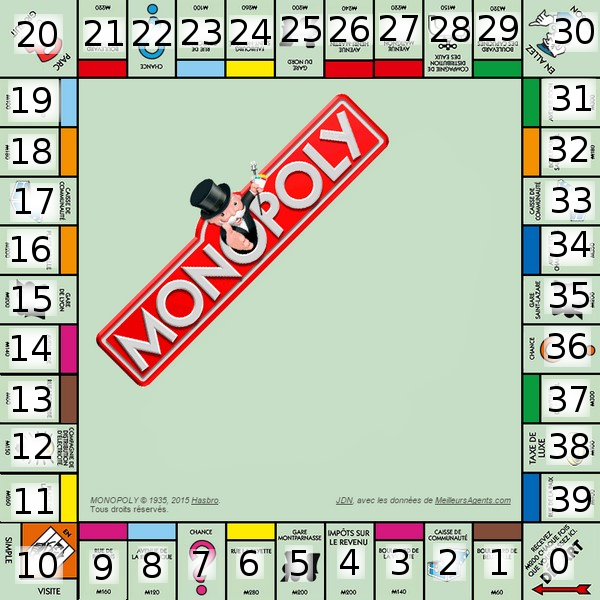
\includegraphics[scale=0.4]{./Images/Monopoly.png}
	\caption{Numérotation du Monopoly (basée sur une image venant du site 
	\cite{IMG_Monopoly})}
    \end{figure}
    
    Chaque déplacement du pion (c'est-à-dire à chaque fois que l'on lance le dé) sera 
    traduit par un changement d'état.
    Dans un premier temps, on modélise donc le Monopoly par 40 cases où chaque case est
    reliée aux $6*n-(n-1)$ cases suivantes à partir de la case $n-1$, où $n$ est le 
    nombre de dé.  Dans le cas précis des règles du Monopoly (donc lorsque $n = 2$), 
    chaque case pourra donc accéder à 11 autres cases.  En effet, le résultat le plus 
    petit pouvant être produit par $n$ dés est de $n$ (tous les dé à 1).
    On devra donc éliminer toutes les $n-1$ cases juste après la case actuelle et le résultat
    le plus grand pouvant être produit par $n$ dés sera de $6*n$ (pour un dé à 6 faces).
    \begin{center}
      \begin{tikzpicture}
        \colornode[text width=1cm] at (0, 0) (c0) {Départ};
        \colornode[text width=0.7cm] at (1.5, 0) (c1) {Case 1};
        \colornode[text width=0.7cm] at (3, 0) (c2) {Case 2};
        \colornode[text width=1cm] at (5.5, 0) (cx) {...};
        \colornode[text width=0.7cm] at (7, 0) (c12) {Case 12};
        
        \drawedge
	  (c0) edge[bend left] node {} (c2)
	  (c0) edge[bend left] node {} (cx)
	  (c0) edge[bend left] node {} (c12)
	  (c1) edge[bend right] node {} (cx)
	  (c1) edge[bend right] node {} (c12);
        
      \end{tikzpicture}
    \end{center}
    Cependant, certaines cases ont un comportement particulier comme par exemple la 
    case \textit{aller en prison}, la case \textit{chance} ou encore la case
    \textit{caisse de communauté}.  Les déplacements possibles à partir de ces cases
    ne sont pas les mêmes que pour les autres cases et seront donc étudiées dans les 
    points suivants.
    
  \subsection{Répartition des dés}
    \label{repart_des}
    Lorsque l'on lance 2 dés, la somme des valeurs des dés n'a pas la même probabilité
    d'apparaître.  Il y a par exemple 3 manières différentes de former la valeur 4 (à 
    savoir: $3+1$, $2+2$ et $1+3$) alors qu'il n'y a qu'une seule manière de former 
    un 2 (à savoir: $1+1$).
    C'est ce que nous illustre la figure \ref{tableau_repartition_des}.  Sur celle-ci,
    on peut voir les cases jaunes aux extrémités qui représentent les valeurs que 
    peuvent prendre chacun des dés.  Les cases bleues nous montrent la somme des valeurs
    de chaque dé.  Cette figure nous montre donc toutes les combinaisons possibles en
    lançant deux dés (et donc toutes les valeurs possibles).  On remarque par exemple
    qu'il y a 4 façons de faire un $5$ alors qu'il n'y a qu'une façon de faire un $2$.
    Cette image nous confirme également bien qu'il y a 36 combinaisons possibles 
    lorsqu'on lance 2 dés.
    \begin{figure}[h]
      \centering
      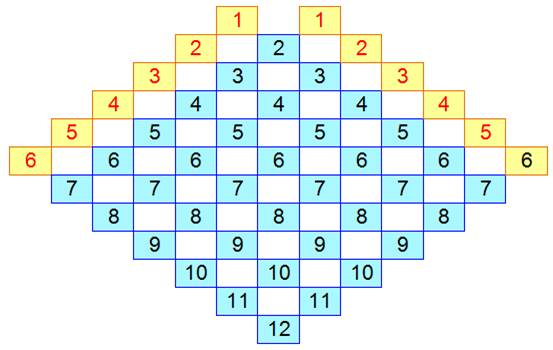
\includegraphics[scale=0.4]{./Images/RepartitionDes.jpg}
	\caption{Répartition des nombres formés avec 2 dés \citep{IMG_Des}}
      \label{tableau_repartition_des}
    \end{figure}
    
    \subsubsection{Calcul de la répartition des dés}
      L'explication intuitive du point \ref{repart_des} peut être généralisée.
      En effet, le Monopoly se joue avec deux dés.  Mais il pourrait être
      intéressant de voir le comportement du jeu avec un autre nombre de dés.
      On va donc s'intéresser à la répartition des valeurs obtenues lorsqu'on 
      lance $n$ dés.  Le site \cite{FORMULE_Des} nous propose la formule 
      suivante:
      $$\sum\limits_{k=0}^{(s-n)/6} (-1)^k \begin{pmatrix}n \\ k\end{pmatrix} 
	\begin{pmatrix}s-6k-1 \\n-1\end{pmatrix}$$
      Où $n$ est le nombre de dés et $s$ le nombre que l'on désire former.
      Pour calculer la répartition totale, il suffit donc d'appliquer cette
      formule à tous les nombres pouvant être formés par $n$ dés.
      Cette équation est basée sur les fonctions génératrices permettant de
      trouver le nombre de combinaisons relatives à la somme de $n$ dés.
      Celle-ci peut donc être utilisée pour calculer la distribution
      des nombres pouvant être formés avec $n$ dés ayant n'importe quel 
      nombre de face et n'importe quel valeur sur ces faces (tant que ce 
      nombre soit naturel).
      Si l'on désire par exemple connaître la répartition d'un dé truqué 
      ayant 3 faces $1$, 5 faces $2$ et une face $3$, on se basera sur le 
      polynôme suivant: $3x + 5x^2 + x^3$.  Pour connaître la distribution 
      des valeurs que l'on peut obtenir en lançant $n$ dés, il suffit de 
      multiplier $n$ fois ce polynôme par lui-même.  Si on lance deux dés,
      on obtient donc:
      \begin{align*}
      &(3x + 5x^2 + x^3)^2\\
      &= (3x \times 3x) + (3x \times 5x^2) + (3x \times x^3) + (5x^2 \times 5x^2) + \\
      \tag*{$(5x^2 \times x^3) + (x^3 \times x^3)$}\\
      &= (9x^2) + (15x^3) + (3x^4) + (25x^4) + (5x^5) + (x^6)\\
      &= 1 x^6 + 5x^5 + 28x^4 + 15x^3 + 9x^2
      \end{align*}
      En faisant la somme des coefficients, on obtient le nombre d'arrangements 
      possibles.  Dans le cas présent, on a donc $1 + 5 + 28 + 15 + 9$ c'est à 
      dire $59$.  En regardant chaque monôme, on peut connaître la répartition
      de chaque valeur formée par le lancé de ces 2 dés truqués.  En effet, 
      l'exposant nous donne le résultat formé et le coefficient permet de 
      connaître sa probabilité.  Pour $9 x^2$ on peut donc déduire que la 
      valeur $2$ aura une probabilité $9/59 = 0.15$ d'avoir lieu, ce même
      raisonnement peut être fait pour chacun des monômes.
      L'équation exprimée au début de ce point représente simplement le 
      développement de ce polynôme.
    
  \subsection{Faire un double}
    Les règles du Monopoly stipulent que lorsque l'on fait 3 doubles 
    consécutifs, on est directement envoyé en prison.
    \subsubsection{Modélisation}
      \label{modelisation_double}
      Pour modéliser ce comportement via une 
      chaîne de Markov, il faut tripler le nombre d'états.  En effet, une case 
      $i$ peut être visitée après avoir fait 0 double, 1 double ou 2 doubles.  
      On peut donc représenter cela comme 3 plateaux de jeux parallèles comme
      montré sur la figure \ref{representation_double}.  A chaque fois que l'on
      fait un double, on se retrouve à un niveau ``plus bas'' (sur l'image).  
      On a donc 3 niveaux: 0 où aucun double n'a encore été fait, 1 où le coup 
      précédent était un double et le niveau 2 où les deux coups précédents 
      étaient des doubles. Lorsque l'on faire un 3\up{ème} double, on se 
      retrouve directement en prison.  Les flèches en rouges sur la figure nous 
      montrent les déplacements faits lorsque l'on obtient trois doubles 
      consécutifs, à savoir dans le cas présent: $1+1$, $2+2$ et $6+6$.  Les 
      flèches bleues nous montrent ce qui se passe lorsque l'on obtient un 
      simple nombre (pas un double).  Elles sont toutes dirigées vers le 
      plateau le plus haut sur l'image, c'est-à-dire celui où l'utilisateur 
      n'a pas encore fait de double.
      \begin{figure}[h]
	\centering
	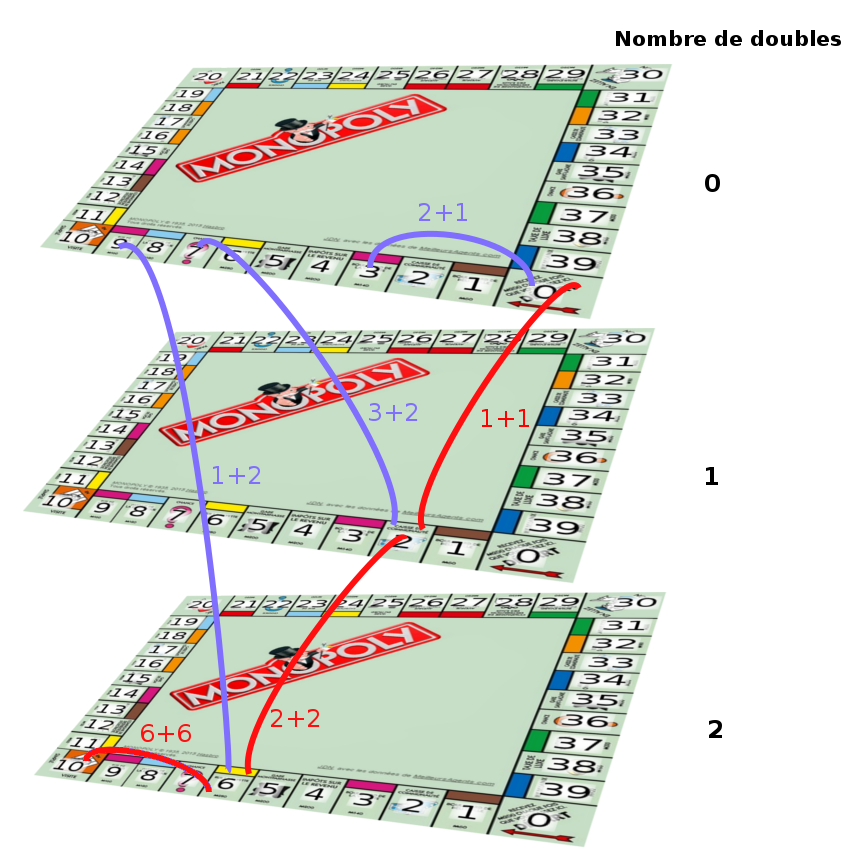
\includegraphics[scale=0.4]{./Images/MonopolyVertical_legende.png}
	  \caption{Déplacement en cas de double}
	  \label{representation_double}
      \end{figure}
    \subsubsection{Probabilité de faire un double}
      \label{prob_double}
      Comme vu dans le point \ref{repart_des}, il serait intéressant de 
      pouvoir modéliser le Monopoly pour $n$ dés.  Il faut donc d'abord
      définir ce qu'est un \textit{double}.  Dans cet article, on va
      considérer que le joueur aura fait un double (au sens du Monopoly)
      si tous les nombres indiqués par les dés sont les mêmes. En d'autres
      mots, ce nombre est donc définit tel que $i*n$ où $i$ est le nombre
      indiqué par tous les dés.  Par définition ce nombre est donc 
      divisible par le nombre de dés.
      Il faut cependant bien tenir compte du fait qu'il y a plusieurs
      manières de former un même nombre.  Par exemple avec deux dés, 
      il y a trois manières différentes de former le nombre $4$: 
      $1+3$, $2+2$ et $3+1$.  Il y a donc 3 chance sur 36 de faire un 
      $4$ mais seulement une chance sur 36 de faire un double.
      Pour une partie de Monopoly classique (où il y a donc seulement
      deux dés), il y a 6 chance sur 36 de faire un double, à savoir:
      $2$, $4$, $6$, $8$, $10$ et $12$.  Chaque double à une chance
      sur 36 d'apparaître.
    
  \subsection{Case \textit{prison}}
    \label{case_prison}
    Les règles du Monopoly stipulent que l'on peut sortir de prison de 
    plusieurs manières différentes: soit via une carte chance, soit en 
    payant, soit en faisant un double. Seul les deux dernières solutions 
    seront utilisées dans cette modélisation. En effet, pour modéliser 
    l'utilisation d'une carte permettant de sortir de prison, il faudrait, 
    comme au point \ref{modelisation_double} dupliquer chaque case 
    pour savoir si on est dans un état où l'on a une carte ou pas.  
    Les règles indiquent également que l'on ne peut rester que 3 tours 
    maximum avant d'être obligé de payer. Afin de représenter ces 
    différentes cas, la case prison sera triplée. On aura donc trois 
    représentations de la case prison: au premier, second et troisième 
    tour. La case \textit{aller en prison} sera donc considérée comme 
    une case prison de niveau 0 et n'aura qu'une seule arête visant la 
    case \textit{prison premier tour}. Comme vu au point \ref{prob_double}, 
    il y a une probabilité de $6/36$ de faire un double.  Dans les 5 
    autres cas sur 6, on doit relancer le dés et on passera sur la case 
    prison \textit{suivante}. Une fois arrivé sur la dernière case 
    prison, on est obligé de payer.\\
    En résumé, il y a 7 déplacements possibles lorsque l'on sort de
    prison:
    \begin{itemize}
      \item faire un double (et avancer du résultat de ce double), 
	ce qui correspond à 6 déplacements;
      \item payer et se retrouver sur la case \textit{prison visite 
	uniquement}.
    \end{itemize}
    
  \subsection{Cases \textit{chance}}
    Les cases chances font piocher une carte dans le paquet des
    cartes \textit{chance}.  On suppose que chaque carte a la 
    même probabilité d'être piochée. Ces cartes peuvent faire gagner de 
    l'argent mais également déplacer les pions présents sur le plateau 
    de jeu.  C'est évidemment ce second comportement qui sera étudié 
    ici.  Le Monopoly comporte 16 cartes chances ayant la répartition 
    suivante:
    \begin{itemize}
     \item 8 cartes faisant référence à des payements;
     \item une carte \textit{sortir de prison};
     \item 7 cartes faisant référence à un déplacement.
    \end{itemize}
    On peut donc en déduire que lorsqu'un joueur pioche une carte 
    chance, il aura une 7 chance sur 16 de devoir déplacer son pion.  
    Ces déplacements sont les suivants:
    \begin{itemize}
     \item reculer de 3 cases;
     \item se rendre à la case départ;
     \item aller en prison;
     \item se rendre à la 11\up{ème} case (où 0 est le départ);
     \item se rendre à la 15\up{ème} case;
     \item se rendre à la 24\up{ème} case;
     \item se rendre à la 36\up{ème} case (dernière case avant l'arrivée).
    \end{itemize}
    Dans les 9 autres cas on lancera simplement les dés.  Les cases 
    chances ont donc beaucoup d'arêtes.
    
  \subsection{Cases \textit{caisse de communauté}}
    Comme les cases \textit{chance}, les cases \textit{caisse de 
    communauté} font piocher une carte du même nom dans les mêmes
    condition que les cartes \textit{chance}.  Les cartes 
    \textit{caisse de communauté} sont plus axées sur l'aspect 
    financier du jeu. Cependant 3 cartes provoquent également des 
    déplacements des pions:
    \begin{itemize}
     \item se rendre à la case départ;
     \item aller en prison;
     \item se rendre sur le première case.
    \end{itemize}
    La modélisation des cases \textit{caisse de communauté} se fait de la 
    même manière que les cases \textit{chance}.
    
  \subsection{Probabilité de visiter une case}
    Comme introduit dans le point \ref{modeliation_monopoly}, le Monopoly
    peut être vu comme une chaîne de Markov et plus particulièrement un
    BSCC.  On va donc utiliser la distribution stationnaire (présentée dans
    le point \ref{distribution_stationnaire}) afin de connaître la
    probabilité de visiter chaque case et en déduire quelle est la case la
    plus visitée.
    
    
\section{Résultat}


\section{Conclusion}
  
  
%     ===== EXEMPLE =====
%     \begin{tikzpicture}
%       % Draw the states
%       \node[state,
% 	    text=yellow,
% 	    draw=none,
% 	    fill=gray!50!black] (s) {Sunny};
%       \node[state,
% 	    right=of s,
% 	    text=blue!30!white, 
% 	    draw=none, 
% 	    fill=gray!50!black] (r) {Rainy};
% 
%       % Connect the states with arrows
%       \draw[every loop]
% 	  (s) edge[bend right] node {} (r)
% 	  (r) edge[bend right] node {} (s)
% 	  (s) edge[bend right, auto=left]  node {0.6} (r)
% 	  (r) edge[bend right, auto=right] node {0.7} (s)
% 	  (s) edge[loop above]             node {0.4} (s)
% 	  (r) edge[loop above]             node {0.3} (r);
%     \end{tikzpicture}
  

\footnotesize
\nocite{*}
\bibliographystyle{apalike}
\bibliography{Rapport}


\end{document}